
\documentclass[11pt]{article}
\usepackage{standalone}
\usepackage[margin=0.75in, headheight=20pt]{geometry}

\usepackage{amsmath}
\usepackage{amsfonts}
\usepackage{amssymb}
\usepackage{mathtools}

\usepackage[utf8]{inputenc}
\usepackage[english]{babel}
\setlength{\parindent}{2em}
\setlength{\parskip}{.25em}
\renewcommand{\baselinestretch}{1.0}

\usepackage{fancyhdr}
\pagestyle{fancy}
\rhead{ Clarke | Blostein | Queen's University}
\renewcommand{\headrulewidth}{0.4pt}
\renewcommand{\footrulewidth}{0.4pt}

\usepackage{courier}

\usepackage[]{algorithm2e}
\usepackage{mathrsfs}

\usepackage{etoolbox}
\patchcmd{\thebibliography}{\chapter*}{\section*}{}{}




\title{Performance Analysis of Semi-Orthogonal User Groups}
\author{J.E. Clarke, Dr. S.D. Blostein | Queen's University}
\date{Summer, 2018}

\begin{document}
	\maketitle
	\newpage
    \section{Maximum Ratio Transmission Beamforming Performance as a Function of a Known Orthogonality Requirement}
    	\subsection{System Model}
            
\begin{figure}
    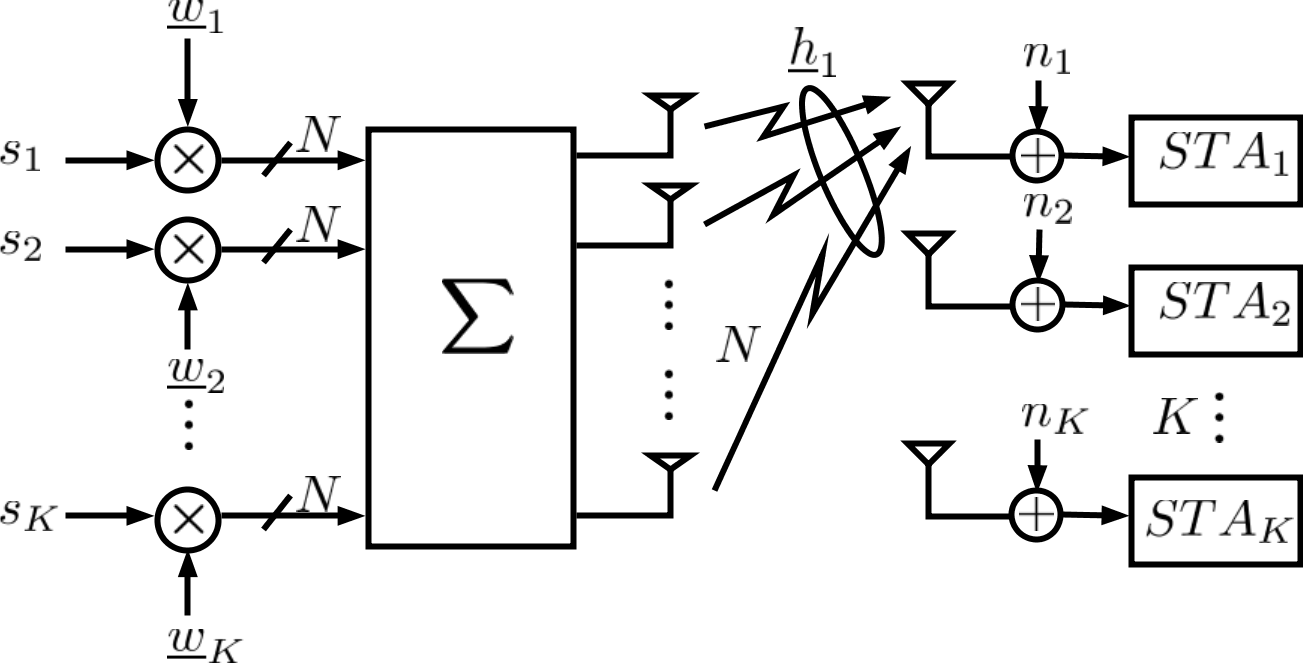
\includegraphics[width=12cm]{figs/system_desc.png}\\
    \caption{Block diagram of the system model.}
    \label{fig:sys_bd}
\end{figure}

        \subsection{MRT Beamforming Scheme, SINR, and Sum Rate Analysis}
        asdf
        \subsection{Experiment Implementation and Results}
        asdf

    \newpage
	\section{Appendices}
	    %\subsection{Notes on Gamma-distributed variables}
	    %    \input{app/gamma_dist.tex}
    \newpage	
 	\begingroup
 		\renewcommand{\section}[2]{}%
 		\bibliographystyle{IEEEtran}
% 		\bibliography{user_sel_lit}
 	\endgroup
\end{document}

Imported from Another project/review.tex, at 3:21 pm Today

 
